\cotefile{161-5}
\scanpage{17}
\mspage{131}
\begin{center}Sur les groupes de Galois attachés aux groupes $p$-divisibles\end{center}

spéciale aux groupes de dimension 1). On en déduit que \textit{$I$ est un sous-groupe ouvert de $G$}; je ne connais pas de démonstration directe de ce fait.

3) Le groupe $I$ possède deux filtrations naturelles $v$ et $w$, définies de la manière suivante:
\[
\begin{aligned}
v(g)&\geqslant n\Leftrightarrow(g-1)(T)\subset p^nT\,,\\
w(g)&\geqslant n\Leftrightarrow g\in I^n
\end{aligned}
\]
($I^n$ désigne le $n$-ème groupe de ramification de $I$, dans la notation supérieure, cf. [\textit{6}], chap. IV, \S~3).

Quelle relation y a-t-il entre $v$ et $w$? Si $e_K$ désigne l’indice de ramification absolu de $K$, est-il vrai que l’on a
\[
w=e_K\cdot v+O(1)\,?
\]
% Right bracket, with a middle stroke, spans the question and the following paragraph.
\margin{\handwritten{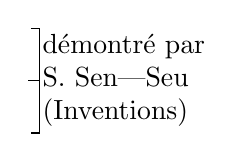
\begin{tikzpicture}[baseline=(n.center)]
\node[align=left,inner sep=0pt] (n) at (0,0) {démontré par\\S. \unsure{Sen|Seu}\\(Inventions)};
\draw ([xshift=-4pt,yshift=2pt]n.north west) -- ([xshift=-1pt,yshift=2pt]n.north west) -- ([xshift=-1pt,yshift=-2pt]n.south west) -- ([xshift=-4pt,yshift=-2pt]n.south west);
\draw ([xshift=-5pt]n.west) -- ([xshift=-1pt]n.west);
\end{tikzpicture}}}
Une question analogue se pose pour tous les groupes de Lie $p$-adiques qui sont des groupes de Galois.

\begin{center}\textbf{Bibliographie}\end{center}

[\textit{1}] \textsc{Chevalley}, C.: Théorie des groupes de LIE, II et III. Publ. Inst. Math. Univ. Nancago, Paris: Hermann 1951 et 1955.

[\textit{2}] \textsc{Lubin}, J.: One-parameter formal LIE groups over $p$-adic integer rings. Ann. of Maths. \textbf{80}, 464--484 (1964).

[\textit{3}] \textsc{Lubin}, J.: Finite subgroups and isogenies of one-parameter formal LIE groups. Ann. of Maths. \textbf{85}, 296--302 (1961).

[\textit{4}] \textsc{Mumford}, D.: Geometric invariant theory. Ergeb. der Math., Neue Folge, Bd. 34. Berlin, Heidelberg, New York, Springer 1965.

[\textit{5}] \textsc{Mumford}, D.: Families of abelian varieties. Algebraic groups and discontinuous subgroups. Proc. Symp. Pure Maths. \textbf{9}, A.M.S. (1966).

[\textit{6}] \textsc{Serre}, J-P.: Corps Locaux. Publ. Inst. Math. Univ. Nancago, VIII, Paris: Hermann 1962.

[\textit{7}] \textsc{Serre}, J-P.: LIE algebras and LIE groups. New York: Benjamin 1965.

[\textit{8}] \textsc{Serre}, J-P.: Résumé des cours 1965--66. Annuaire du Collège de France, 49--58, (1966--67).

[\textit{9}] \textsc{Tate}, J.: $p$-divisible groups, ce volume p. 158--183.
% archive sheet number: 16
